\documentclass{sig-alternate}

\begin{document}
%
% --- Author Metadata here ---
\conferenceinfo{WOODSTOCK}{'97 El Paso, Texas USA}
%\CopyrightYear{2012} % Allows default copyright year (20XX) to be over-ridden - IF NEED BE.
%\crdata{0-12345-67-8/90/01}  % Allows default copyright data (0-89791-88-6/97/05) to be over-ridden - IF NEED BE.
% --- End of Author Metadata ---

\title{Cartographic documents for web modeling and representation of indoor mapping with interactive environments}
\subtitle{[Extended Abstract]
\titlenote{A full version of this paper is available as
\emph{Author's Guide to Preparing ACM SIG Proceedings Using
\LaTeX$2_\epsilon$\ and BibTeX} at
\texttt{www.acm.org/eaddress.htm}}}
%
% You need the command \numberofauthors to handle the 'placement
% and alignment' of the authors beneath the title.
%
% For aesthetic reasons, we recommend 'three authors at a time'
% i.e. three 'name/affiliation blocks' be placed beneath the title.
%
% NOTE: You are NOT restricted in how many 'rows' of
% "name/affiliations" may appear. We just ask that you restrict
% the number of 'columns' to three.
%
% Because of the available 'opening page real-estate'
% we ask you to refrain from putting more than six authors
% (two rows with three columns) beneath the article title.
% More than six makes the first-page appear very cluttered indeed.
%
% Use the \alignauthor commands to handle the names
% and affiliations for an 'aesthetic maximum' of six authors.
% Add names, affiliations, addresses for
% the seventh etc. author(s) as the argument for the
% \additionalauthors command.
% These 'additional authors' will be output/set for you
% without further effort on your part as the last section in
% the body of your article BEFORE References or any Appendices.

\numberofauthors{8} %  in this sample file, there are a *total*
% of EIGHT authors. SIX appear on the 'first-page' (for formatting
% reasons) and the remaining two appear in the \additionalauthors section.
%
\author{
% You can go ahead and credit any number of authors here,
% e.g. one 'row of three' or two rows (consisting of one row of three
% and a second row of one, two or three).
%
% The command \alignauthor (no curly braces needed) should
% precede each author name, affiliation/snail-mail address and
% e-mail address. Additionally, tag each line of
% affiliation/address with \affaddr, and tag the
% e-mail address with \email.
%
% 1st. author
\alignauthor
Ben Trovato\titlenote{Dr.~Trovato insisted his name be first.}\\
       \affaddr{Institute for Clarity in Documentation}\\
       \affaddr{1932 Wallamaloo Lane}\\
       \affaddr{Wallamaloo, New Zealand}\\
       \email{trovato@corporation.com}
% 2nd. author
\alignauthor
G.K.M. Tobin\titlenote{The secretary disavows
any knowledge of this author's actions.}\\
       \affaddr{Institute for Clarity in Documentation}\\
       \affaddr{P.O. Box 1212}\\
       \affaddr{Dublin, Ohio 43017-6221}\\
       \email{webmaster@marysville-ohio.com}
% 3rd. author
\alignauthor Lars Th{\o}rv{\"a}ld\titlenote{This author is the
one who did all the really hard work.}\\
       \affaddr{The Th{\o}rv{\"a}ld Group}\\
       \affaddr{1 Th{\o}rv{\"a}ld Circle}\\
       \affaddr{Hekla, Iceland}\\
       \email{larst@affiliation.org}
\and  % use '\and' if you need 'another row' of author names
% 4th. author
\alignauthor Lawrence P. Leipuner\\
       \affaddr{Brookhaven Laboratories}\\
       \affaddr{Brookhaven National Lab}\\
       \affaddr{P.O. Box 5000}\\
       \email{lleipuner@researchlabs.org}
% 5th. author
\alignauthor Sean Fogarty\\
       \affaddr{NASA Ames Research Center}\\
       \affaddr{Moffett Field}\\
       \affaddr{California 94035}\\
       \email{fogartys@amesres.org}
% 6th. author
\alignauthor Charles Palmer\\
       \affaddr{Palmer Research Laboratories}\\
       \affaddr{8600 Datapoint Drive}\\
       \affaddr{San Antonio, Texas 78229}\\
       \email{cpalmer@prl.com}
}
% There's nothing stopping you putting the seventh, eighth, etc.
% author on the opening page (as the 'third row') but we ask,
% for aesthetic reasons that you place these 'additional authors'
% in the \additional authors block, viz.
\additionalauthors{Additional authors: John Smith (The Th{\o}rv{\"a}ld Group,
email: {\texttt{jsmith@affiliation.org}}) and Julius P.~Kumquat
(The Kumquat Consortium, email: {\texttt{jpkumquat@consortium.net}}).}
\date{30 July 1999}
% Just remember to make sure that the TOTAL number of authors
% is the number that will appear on the first page PLUS the
% number that will appear in the \additionalauthors section.

\maketitle
\begin{abstract}
PUT THE ABSTRACT HERE
\end{abstract}

% A category with the (minimum) three required fields
\category{H.4}{Information Systems Applications}{Miscellaneous}
%A category including the fourth, optional field follows...
\category{D.2.8}{Software Engineering}{Metrics}[complexity measures, performance measures]

\terms{Theory}

\keywords{ACM proceedings, \LaTeX, text tagging}

\section{Introduciton}\label{introduciton}

\ldots{}

The remainder of the paper is organized as follows. In Section II is
provided an overview of the state of the art. Section III is devoted to
describe the novel cartographic document proposed, while section IV
introduces the underlying mathematical structure. Section V reports
about the tools and instruments developed specifically for the web,
focusing on software architecture, implemented algorithms and real
applications. Section VI describes one use case of both document format
and software tools. Finally Section VII proposes some conclusive remarks
and future developments.

\section{State of the art}\label{state-of-the-art}

PUT THE STATE OF THE ART HERE

\subsection{GeoJSON}\label{geojson}

GeoJSON is a format for encoding a variety of geographic data
structures. GeoJSON supports the following geometry types:
\texttt{Point}, \texttt{LineString}, \texttt{Polygon},
\texttt{MultiPoint}, \texttt{MultiLineString}, and
\texttt{MultiPolygon}. Lists of geometries are represented by a
\texttt{GeometryCollection}. Geometries with additional properties are
\texttt{Feature} objects. And lists of features are represented by a
\texttt{FeatureCollection}.
\href{GeoJSON\%20spec}{http://geojson.org/geojson-spec.html}

GeoJSON is good for geographic mapping application, but not for indoor
application. There is a GeoJSON variant suitable for indoor app.

\subsection{Experiences on Indoor
JSON}\label{experiences-on-indoor-json}

\texttt{IndoorJSON} is a GeoJSON variant used by indoor.io toolset to
define indoor maps. IndoorJSON may consist of any number of Features
and/or FeatureCollections. All Features are interpreted similarly
regardless of their grouping into nested FeatureCollections. IndoorJSON
supports all GeoJSON geometry types.

\section{Advances on cartographics document standards:
HIJSON}\label{advances-on-cartographics-document-standards-hijson}

\textbf{HIJSON} (\textbf{H}ierarchical \textbf{I}ndoor \textbf{JSON}) is
a GeoJSON variant. A HIJSON document reveals at least three major
enhancements above the actual state of the art in indoor cartographic
documents:

\begin{enumerate}
\def\labelenumi{\arabic{enumi}.}
\itemsep1pt\parskip0pt\parsep0pt
\item
  Hierarchical structure
\item
  Metric local coordinate System
\item
  Semantic extensions
\end{enumerate}

\subsubsection{Hierarchical structure}\label{hierarchical-structure}

Unlike other formats like GeoJSON or IndoorJSON, HIJSON organizes its
elements in a hierarchical structure, where every element represent a
potential container for other elements. This structure allows a clear
and logical organization of the elements inside the structure, and at
the same time make it possible to use a relative, local, metric
coordinates system.

\subsubsection{Metric local coordinate System}\label{metric-local-coordinate-system}

In GeoJSON all the positions are expressed in geographical coordinates
(usually WGS84). Although this can be useful for outdoor geographical
representations, it is not the best solution for indoor descriptions. In
HIJSON all the coordinates are expressed in a relative system based on
the hierarchical structure. The shape of all elements is described
starting from origin, and then two vectors (translation and rotation)
describe the position relative to the origin of the parent element. By
this way it is possible to describe the position of a piece of furniture
by specifying its distance from the origin of the room, that is
obviously more convenient than describing its geographical coordinates.
Another advantage is represented by the adoption of a metric reference.
A recursive process that computes intermediate transformation matrixes
can then produce a standard GeoJSON representation, that can be
visualized on any standard viewer.

\subsubsection{Semantic extensions}\label{semantic-extensions}

Every HIJSON Element has a property that describes its class. This
information allows the adoption of semantic extensions by the software
that manipulates the HIJSON data. In the Javascript library developed to
manage HIJSON documents, different classes are instantiated to represent
HIJSON Nodes, which acts differently by the adoption of polymorphic
methods. Ino rder to extend the possibilities in representation and
interaction, it is sufficient to define new classes that reflects new
categories of HIJSON Elements.

\section{LAR: the underlying mathematical structure}\label{lar-the-underlying-mathematical-structure}

\section{Implemented web tools}\label{implemented-web-tools}

A set of web based instruments has been developed allowing to deal with
the HIJSON document previously described. Tools are written in
\emph{JavaScript} language, using \emph{Node.js} and in particular
\emph{Express.js} as backend framework, and exploiting the power of
WebSocket protocol through the \emph{Socket.io} library.

\subsection{Architecture}\label{architecture}

The overall architecture of the tools are, as for the vast majority of
the web based application, inherently \emph{client/server}.

\subsubsection{HIJSON processing pipeline}\label{hijson-processing-pipeline}

Each time a new HIJSON document is submitted to the server, it is passed
through the \textbf{HIJSON processing pipeline}, where it is subjected
to a sequence of preliminary transformations.

The application of the transformation pipeline has a double aim. The
first one consists in generating the graph of valid paths between all
the interesting HIJSON elements. The second aim is the generation of one
\emph{GeoJSON} document for each story of the building described by the
HIJSON document. In this way any connected client can be provided with a
bidimensional plant for each level of the building that it can visualize
through any compliant GeoJSON viewer.

HIJSON processing pipeline (as pictured in figure \ldots{}) is composed
by 6 elaboration stages. In the following are detailed operations
excecuted by each stage, which are, in the order: \emph{validation},
\emph{georeferencing}, \emph{parsing}, \emph{graph paths generation},
\emph{2D layers generation}, \emph{marshalling}.

\begin{figure}
\centering
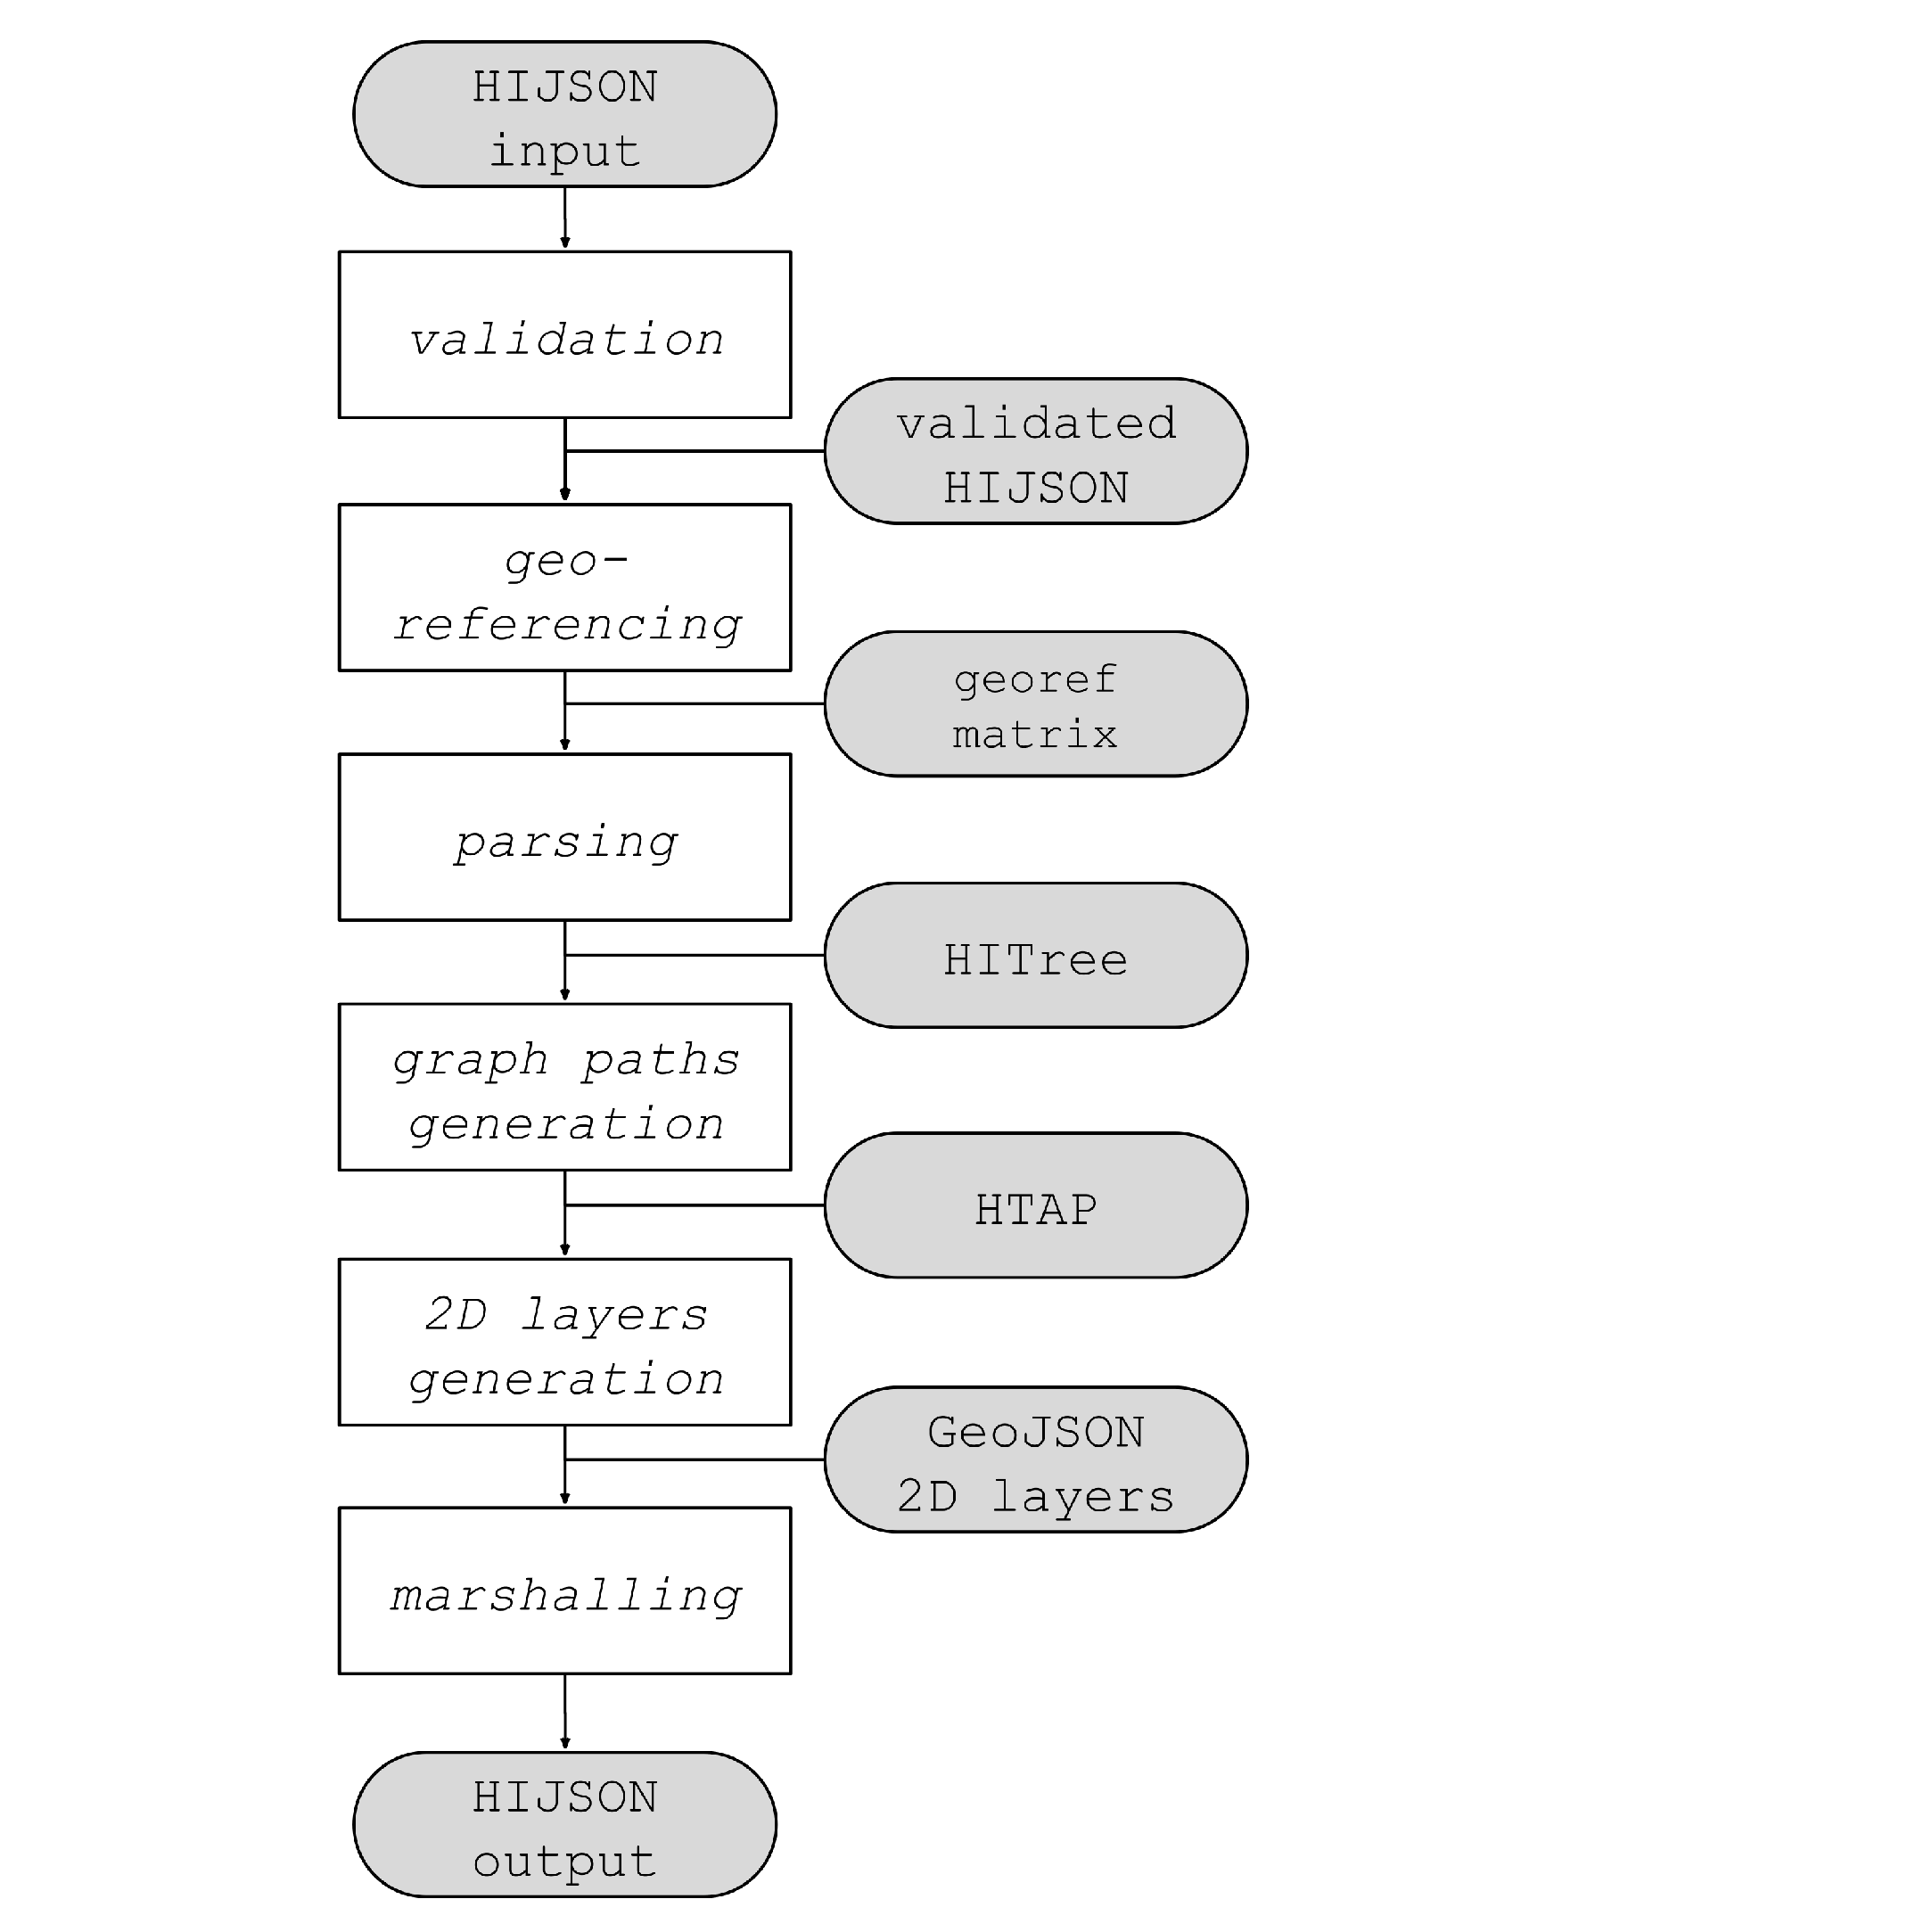
\epsfig{file=images/pipeline.eps, height=3.5in}
\caption{HIJSON processing pipeline}
\label{fig:pipeline}
\end{figure}

1. {[}\textbf{validation}{]} - The first one is a validation stage. In
order to begin with the effective transformations the input HIJSON
document must be compliant with the rules defined in (AGGIUNGERE REF TO
PARAGRAFO REGOLE DI VALIDITA'). In the case the validation stage fails,
processing aborts and do not continue to following stages. If the stage
success, the output for the next stage is a validated HIJSON. 2.
{[}\textbf{georeferencing}{]} - 3. {[}\textbf{parsing}{]} - The parsing
stage, takes the validated HIJSON as its input, that as illustrated
before can be thought of as a list of HIJSON Elments, parses them and
produce an istance of HITREE, which is an object in memory representing
the tree hierarchical structure of the building described into the
HIJSON. 4. {[}\textbf{graph paths generation}{]} - The fourth stage is
in charge of THE generatio of the graph paths. This aim is accomplished
according to the algorithm described in (AGGIUNGERE RIFERIMENTO A
\#\#\#\# Automatic generation of valid paths). The graph paths will be
useful afterwards to coumpute valid paths from couple of point of
interest on the graph. Once the graph paths has been computed, the input
HITREE is augmented with paths information, becoming what has been
called an HTAP (HITREE Augmented with Paths). Augmentation always takes
place as leaf nodes added as children of a specific (e.g. ``room'')
level. 5. {[}\textbf{2D layers generation}{]} - The fifth state is the
generation of geoJSON layer. For each level, the system generates one
geoJSON layer that will be use for the creation of 2D map. Each layer
contains the children of `level' node in the HITREE. Every class
contains a boolean value that is use to choose which class will be a
part of geoJSON layer. Every element has a geographical coordinates
calculated by the transformation matrix with regard to the local
coordinates of the HIJSON element. 6. {[}\textbf{marshalling}{]} -

\subsubsection{Client}\label{client}

When a client connects to the server, it receives the HIJSON input
files, the ready-to-use GeoJSON layers and the weighted adjacency matrix
of the grapth paths. A very short pipeline of processing is performed by
the client, composed by: 1. {[}\textbf{Parsing}{]} - Like for the
Server-side processing, the HIJSON Elements in the input files are
processed and tranformed in HIJSON Nodes, linked together in a
hierarchical tree structure. 2. {[}\textbf{3D Model generation}{]} -
Unlike HIJSON Elements (that are simple Javascript objects), HIJSON
Nodes are instances of specific classes, representing a particular
category of element in the building. Through a polymorphic method, each
node generates a Three.js 3D model of its entity, that is used to
assemble a complete 3D Model of the building. The similarities in HIJSON
hierarchical structure and Three.js scene graph allow this process to be
performed with little effort.

\subsection{Algorithmics}\label{algorithmics}

\subsubsection{Automatic generation of valid
paths}\label{automatic-generation-of-valid-paths}

One of the core functionalities of the pre-processing server stage is
the generation of a graph of valid paths trough the entire building,
that can be used to calculate directions between two given nodes (see
Crossfloor user navigation paragraph). Taking advantage of the
hierarchical structure of the representation, the problem is splitted in
many sub-problems represented by the computation of the sub-graphs
relative to each room. The sub-graphs are then linked together trough
doors. The entire process (as shown in figure), is composed by 4 phases:
1. Computation of the walkable area of the room; 2. Triangulation of the
walkable area; 3. For each triangle side completely internal to the
area, its midpoint is used to represent a graph node; 4. Nodes relative
to the same triangle are then linked together, and the doors are linked
to the nearest node in the room.

\begin{figure*}[htbp] % figure placement: here, top, bottom, or page
  \centering
  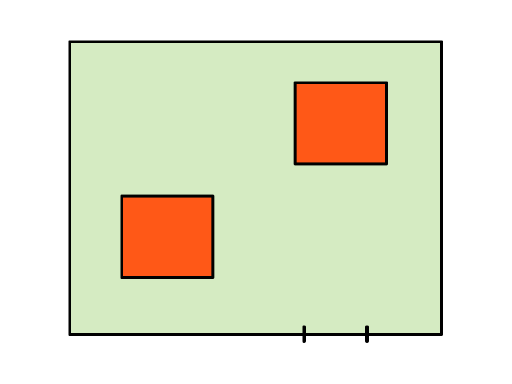
\includegraphics[height=0.2\linewidth,width=0.2425\linewidth]{images/graph-generation-1}
  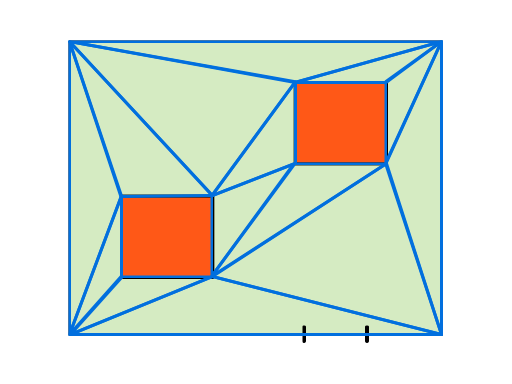
\includegraphics[height=0.2\linewidth,width=0.2425\linewidth]{images/graph-generation-2}
  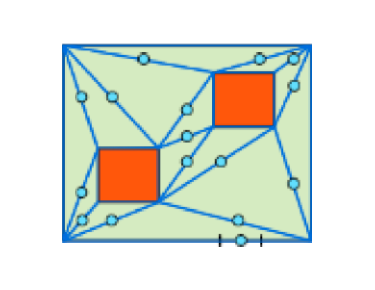
\includegraphics[height=0.2\linewidth,width=0.2425\linewidth]{images/graph-generation-3}
  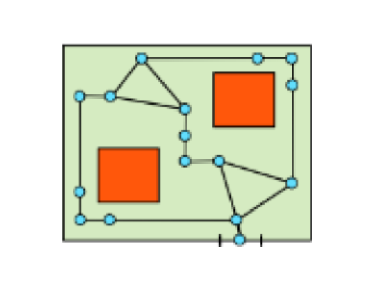
\includegraphics[height=0.2\linewidth,width=0.2425\linewidth]{images/graph-generation-4}
  \caption{Graph paths generation. (a) detection of obstacles; (b) triangulation of walkable area; (c) identification of graph nodes area; (d) junction of nodes.}
  \label{fig:graph-generation}
\end{figure*}


After that, the objects in the room are linked to the graph nodes as
well, giving the possibility to calculate paths to specific elements of
interest. Given the nature of this process, the paths calculated may not
be absolutely optimal, but this strategy ensures a good ratio between
extension of exploration and number of graph nodes.

\subsection{Applications}\label{applications}

\subsubsection{IoT monitoring}\label{iot-monitoring}

Every element in 2D map or in 3D model is interactive and the user can
ask for information. In every class there is a method that gets
information and send that to the client. The modularity of \emph{nome
del software} permits to show particular information with regard to the
object. There are two groups of objects: simple and smart. If the object
is smart, it can send data in real time through its sensor (e.g.~if the
object is a thermostat, the user can see the temperature in the room and
can turn on, or off, the heating). If the object isn't smart, the system
can show static information (e.g.~for fire Extinguisher, the system
shows the last date of checking).

\subsubsection{Realtime access
monitoring}\label{realtime-access-monitoring}

The system can be used for access monitoring. On 2D map will be a marker
for each person in the building, whereas on the 3D model will be a 3D
model of user. With an appropriate system of indoor localization, every
person sends its position in real time. The 2D map and the 3D model is
automatically refreshed. The user can ask for information about person,
in function of the use of the system.

\subsubsection{Crossfloor user
navigation}\label{crossfloor-user-navigation}

With the weighted adjacency matrix, the user can choose two nodes that
represent respectively the start and the end point. The system
calculates the optimal path by Dijkstra's algorithm and shows this with
a polyline in 2D map. To pass through different floors, the path leads
to stairs or elevators. All the nodes of the same elevator are connected
among them and their distances is set to 0. Otherwise the connections
through the stairs are characterized by the nodes of two different
levels; their weight of this portion of path is set to the distance
between these nodes. Therefore the subgraph that characterized stairs or
elevator is complete.

\section{Use case}\label{use-case}

\begin{verbatim}
C3D.js
\end{verbatim}

\section{Conclusions}\label{conclusions}

We presented HIJSON a GeoJSON extension for indoor mapping

%ACKNOWLEDGMENTS are optional
\section{Acknowledgments}
This section is optional; it is a location for you
to acknowledge grants, funding, editing assistance and
what have you.  In the present case, for example, the
authors would like to thank Gerald Murray of ACM for
his help in codifying this \emph{Author's Guide}
and the \textbf{.cls} and \textbf{.tex} files that it describes.

%
% The following two commands are all you need in the
% initial runs of your .tex file to
% produce the bibliography for the citations in your paper.
\bibliographystyle{abbrv}
\bibliography{sigproc}  % sigproc.bib is the name of the Bibliography in this case
% You must have a proper ".bib" file
%  and remember to run:
% latex bibtex latex latex
% to resolve all references
%
% ACM needs 'a single self-contained file'!
%
%APPENDICES are optional
%\balancecolumns
\appendix
%Appendix A
\section{Headings in Appendices}
The rules about hierarchical headings discussed above for
the body of the article are different in the appendices.
In the \textbf{appendix} environment, the command
\textbf{section} is used to
indicate the start of each Appendix, with alphabetic order
designation (i.e. the first is A, the second B, etc.) and
a title (if you include one).  So, if you need
hierarchical structure
\emph{within} an Appendix, start with \textbf{subsection} as the
highest level. Here is an outline of the body of this
document in Appendix-appropriate form:
\subsection{Introduction}
\subsection{The Body of the Paper}
\subsubsection{Type Changes and  Special Characters}
\subsubsection{Math Equations}
\paragraph{Inline (In-text) Equations}
\paragraph{Display Equations}
\subsubsection{Citations}
\subsubsection{Tables}
\subsubsection{Figures}
\subsubsection{Theorem-like Constructs}
\subsubsection*{A Caveat for the \TeX\ Expert}
\subsection{Conclusions}
\subsection{Acknowledgments}
\subsection{Additional Authors}
This section is inserted by \LaTeX; you do not insert it.
You just add the names and information in the
\texttt{{\char'134}additionalauthors} command at the start
of the document.
\subsection{References}
Generated by bibtex from your ~.bib file.  Run latex,
then bibtex, then latex twice (to resolve references)
to create the ~.bbl file.  Insert that ~.bbl file into
the .tex source file and comment out
the command \texttt{{\char'134}thebibliography}.
% This next section command marks the start of
% Appendix B, and does not continue the present hierarchy
\section{More Help for the Hardy}
The sig-alternate.cls file itself is chock-full of succinct
and helpful comments.  If you consider yourself a moderately
experienced to expert user of \LaTeX, you may find reading
it useful but please remember not to change it.
%\balancecolumns % GM June 2007
% That's all folks!
\end{document}
